\documentclass[tikz,border=4pt]{standalone}
\usepackage{libertinus}
\usepackage{amsmath}
\usetikzlibrary{
  arrows.meta,
  backgrounds,
  calc,
  decorations.markings,
  fit,
  positioning
}

\definecolor{accent}{RGB}{38,103,115}
\definecolor{softgray}{RGB}{244,245,246}
\definecolor{midgray}{RGB}{123,128,132}

\tikzset{
  >={Latex[length=2.2mm,width=1.5mm]},
  flow/.style={-Latex,semithick,draw=black!72},
  accent flow/.style={-Latex,semithick,draw=accent},
  box/.style={
    draw=black!68,
    fill=softgray,
    rounded corners=1.2pt,
    align=center,
    inner xsep=5pt,
    inner ysep=4pt
  },
  accent box/.style={
    draw=accent,
    fill=accent!8,
    rounded corners=1.2pt,
    align=center,
    inner xsep=5pt,
    inner ysep=4pt
  },
  point/.style={circle,draw=black!75,fill=white,inner sep=1.7pt},
  accent point/.style={circle,draw=accent,fill=accent!10,inner sep=1.7pt},
  tinylabel/.style={font=\scriptsize,align=center},
  smalllabel/.style={font=\small,align=center},
  panel/.style={draw=black!28,rounded corners=2pt,inner sep=6pt}
}


\tikzset{
  old arc/.style={draw=black!55,semithick},
  boundary A/.style={draw=black,very thick},
  boundary B/.style={draw=accent,very thick,densely dashed},
  new arc/.style={draw=accent,line width=1.2pt},
  value/.style={circle,draw=black!75,fill=white,inner sep=0pt,
                minimum size=4mm,font=\small},
  pending/.style={value,dashed,text=black!60},
  heading/.style={anchor=west,font=\bfseries\small},
  note/.style={anchor=west,font=\small,inner sep=0pt}
}
% x-coordinates are the axis values. All lower-family arcs are drawn in full:
% P3 joins 2 and 8, P5 joins 5 and 7, P7 joins 3 and 4.
\newcommand{\skeleton}[2]{%
  \draw[black!45] (.65,0) -- (8.35,0);
  \draw[old arc] (2,0) arc[start angle=180,end angle=360,x radius=3,y radius=.95];
  \draw[old arc] (5,0) arc[start angle=180,end angle=360,x radius=1,y radius=.52];
  \draw[old arc] (3,0) arc[start angle=180,end angle=360,x radius=.5,y radius=.32];
  \draw[#1] (1,0) arc[start angle=180,end angle=0,x radius=.5,y radius=.53];
  \draw[#2] (4,0) arc[start angle=180,end angle=0,x radius=.5,y radius=.53];
  \draw[old arc] (7,0) arc[start angle=180,end angle=0,x radius=.5,y radius=.53];
}
\newcommand{\newpair}{%
  \draw[new arc] (3,0) arc[start angle=180,end angle=0,x radius=1.5,y radius=.95];
  \node[above,font=\small] at (4.5,.97) {$N=P_8$};
}
% The separate row keeps the point IDs clear of the lower arcs.
\newcommand{\points}[1]{%
  \foreach \x/\idx in {1/1,2/2,3/7,4/6,5/5,6/8,7/4,8/3}{
    \ifnum\x=6 \node[#1] (p\x) at (\x,0) {\x};
    \else \node[value] (p\x) at (\x,0) {\x}; \fi
    \node[font=\small] at (\x,-1.17) {$z_{\idx}$};
  }
}
\newcommand{\panelhead}[1]{%
  \draw[black!28,rounded corners=2pt] (.38,-2.51) rectangle (8.62,2.00);
  \node[heading] at (.55,1.72) {#1};
}
\begin{document}
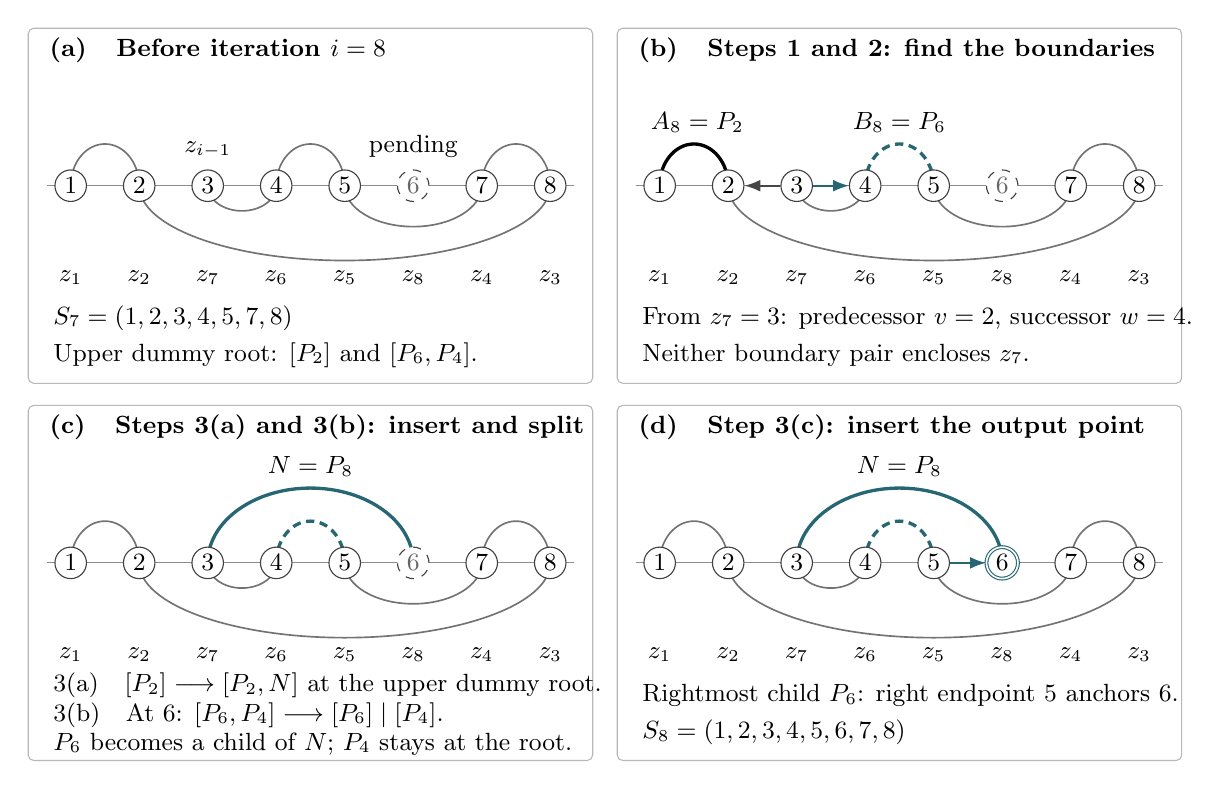
\begin{tikzpicture}[x=.87cm,y=1cm]
  \begin{scope}
    \panelhead{(a)\quad Before iteration $i=8$}
    \skeleton{old arc}{old arc}
    \points{pending}
    \node[above,font=\small] at (3,.23) {$z_{i-1}$};
    \node[above,font=\small] at (6,.23) {pending};
    \node[note] at (.74,-1.68) {$S_7=(1,2,3,4,5,7,8)$};
    \node[note] at (.74,-2.15) {Upper dummy root: $[P_2]$ and $[P_6,P_4]$.};
  \end{scope}
  \begin{scope}[xshift=7.48cm]
    \panelhead{(b)\quad Steps 1 and 2: find the boundaries}
    \skeleton{boundary A}{boundary B}
    \points{pending}
    \draw[flow] (p3.west) -- (p2.east);
    \draw[accent flow] (p3.east) -- (p4.west);
    \node[above,font=\small] at (1.55,.55) {$A_8=P_2$};
    \node[above,font=\small] at (4.5,.55) {$B_8=P_6$};
    \node[note] at (.74,-1.68) {From $z_7=3$: predecessor $v=2$, successor $w=4$.};
    \node[note] at (.74,-2.15) {Neither boundary pair encloses $z_7$.};
  \end{scope}
  \begin{scope}[yshift=-4.79cm]
    \panelhead{(c)\quad Steps 3(a) and 3(b): insert and split}
    \skeleton{old arc}{boundary B}
    \newpair
    \points{pending}
    \node[note] at (.74,-1.56) {3(a)\quad $[P_2]\longrightarrow[P_2,N]$ at the upper dummy root.};
    \node[note] at (.74,-1.93) {3(b)\quad At $6$: $[P_6,P_4]\longrightarrow[P_6]\mid[P_4]$.};
    \node[note] at (.74,-2.30) {$P_6$ becomes a child of $N$; $P_4$ stays at the root.};
  \end{scope}
  \begin{scope}[xshift=7.48cm,yshift=-4.79cm]
    \panelhead{(d)\quad Step 3(c): insert the output point}
    \skeleton{old arc}{boundary B}
    \newpair
    \points{value,double,draw=accent}
    \draw[accent flow] (p5.east) -- (p6.west);
    \node[note] at (.74,-1.68) {Rightmost child $P_6$: right endpoint $5$ anchors $6$.};
    \node[note] at (.74,-2.15) {$S_8=(1,2,3,4,5,6,7,8)$};
  \end{scope}
\end{tikzpicture}
\end{document}
